\documentclass[12pt,letterpaper]{memoir}
\usepackage[utf8]{inputenc}
\usepackage{amsmath}
\usepackage{amsfonts}
\usepackage{amssymb}
\usepackage{graphicx}
\usepackage{times}
\usepackage{geometry}
\geometry{margin=1in}
\renewcommand{\baselinestretch}{2}

\begin{document}
    \vspace*{-50pt}
    \begin{center}
    	\textbf{{\large Dependency Structures in Momentum and Value Strategies}}
    	\\
    	\textit{Alex Garland, Emily Bazcyk, Group 10}
    \end{center}
    
\subsection*{Introduction}
Since their introduction as trading strategies, value and momentum have both been of particular interest to those in the finance community. They each have their own benefits and drawbacks. For value, it can be a sometimes underwhelming performance, while momentum has the "elevator-escalator" pattern, wherein it can face catastrophic losses in a short period of time. While there have been attempts to help combat these failings of the strategies (for instances, see attempts by Moskowitz to limit this effect by using conditional Sharpe Ratio or static volatility strategies), it seems that one of the best ways to avoid this problem is by simply using a combination of the two strategies. It is not immediately apparent (either mathematically or economically) why such a strategy works as well as it does. This paper will attempt to explore one aspect of the underlying mathematics, connect it with economic intuition, and mention possible financial implications of this.
\subsection*{Data, Methodology, and Model}
We begin first by pulling Fama-French factors from Kenneth French's webpage, and using these as a reasonable stand-in for what a momentum or value investor might see in his/her returns. The data is particularly useful, given that there are publicly available daily returns dating back to 1926.

From here, we now create a "combined" strategy by equal weighting the returns from the HML (value) factor, and the momentum factor. All 3 of these strategies show significant autocorrelation, and are thus modeled as an ARMA(5,5) process. A Box-Ljung test confirms that the residuals from this process are prime candidates for GARCH modeling. Given this, we then simulate the residuals as a exponential GARCH(5,5) process with innovations drawn from a skewed Student's t distribution (given that we often find that financial data has quite fat tails).

It is here that we begin to make use of copulas as a means of understanding the underlying statistic, and we have three sets of data that we may fit copulas to. First, we can fit a bivariate copula to the observed monthly returns of momentum and value; secondly, we can fit a bivariate copula to the residuals of the ARMA process; finally, we can fit a bivariate copula to the standardized residuals provided by our eGARCH process. We choose to fit bivariate t-copulas to these processes, as this will allow for the calculation of a tail dependency parameter, a parameter with specific economic and financial implications (that will be explained in further detail later).
\subsection*{Results}
Having now explained the process at hand, we can now explain the particular results from each step of the way. Looking first at the construction of the data, our results confirm those of Moskowitz; the equal weighted value strategy does indeed seem a better strategy than either one of the two, given it's dramatically reduced risk profile. We can see that this is also in line with table 2, a chart measuring the correlation of the two strategies (and their combination). Given the negative correlation between momentum and value, it is easy to see that the combination diversifies away a lot of the risk.

However, just as interesting (if not more so) than the correlation table are the exact specifics of the pseudo-observations (the observations when combined by the empirical cumulative distribution function) of momentum and value, particularly when plotted against each other. This is exactly what is seen in Figure 1. What is most surprising about Fig. 1, though, is the "x" shaped pattern that appears (all of the corners are filled out). It is less common, in other words, that we see a day where one performed on the extreme, and the other did not. This scene is repeated in Fig. 2, implying that when we get extreme errors in our time series predictions, we seem to also get extreme errors in our time series predictions with the other.

The exception, however, seems to be the standardized residuals. The "x" pattern is less pronounced in this chart, which also keeps in line with estimated tail dependency parameters (the observations return an upper/lower tail parameter of .189, the residuals return .192, and the standardized residuals return .106). This is a slightly anomaly and likely deserves future consideration and study in the causal mechanisms.
\subsection*{Economic Implications}
So what are the economic and financial implications of this project? Going point by point, we can see that Figures 1 and 2 and the particular "x" pattern that appears in both of the scatterplot of their observations helps explain one of the particularities of the value-momentum strategy; extreme observations for one means extreme observations for the others. This keeps in line with the behavior shown in previous studies that note an anomalously high return during the Great Recession while noting a much more average return during the subsequent recovery. The causal mechanisms behind this remain unknown, but it is a trend that remains on the daily level and a trend that applies even to error of time series models. This behavior could be beneficial for fund managers, given that they are appropriately appraised of the tendencies for extremes to lead to extremes (as there was, after all, some tendency for clustering at the level of extremely disappointing returns/errors for both strategies at the same time).

However, the real draw for fund managers would likely come from the low tail dependency parameter of the standardized residuals and Figure 3. This largely (but not entirely) removes one level of risk that fund managers could be worried about. Exogenous shocks to each strategy typically won't be affecting each other, which makes the combination strategy a particularly attractive one (because it implies that one can, at least on some level, predict those times when volatility will move together between the two strategies). Thus the dependency structures only weakly persist into the level of randomness. This reduced level of worry about correlation of shock could have a particularly large effect for those managers committed to certain levels of risk, reducing rebalancing costs. It is worth noting, however, that we find a weak persistence, not a complete lack of persistance. In fact, the persistence seems to be more pronounced than a simple measure of correlation might suggest (see Table 3 for a reference to the extremely low stated correlation of standardized residuals).
\subsection*{Robustness and Errors}
Finally, we take a quick look at the robustness of our results and the possibility of error within them. As mentioned before, we made use of an ARMA(5,5)-GARCH(5,5) model, and the vast majority of our coefficients registered statistically significant values, even when considering robust standard errors (as seen in Tables 4 and 5). This is less true for our evaluation on the value strategy than for the momentum strategy, but we are pleased with the results. Even further, a quantile-quantile plot of our standardized residuals supports our skewed t-distribution choice, especially for value (see Figs. 4 and 5). 

With that said, there can still be some concern over the fitting of our model. Box-Ljung tests on the standardized residuals still suggest that there is significant autocorrelation among them. We chose not to fit higher degree models given both the computational expense and the risks of overfitting. Despite even this, we have reason to believe that the results and dependency structures should not change significantly given higher order models. 

The final concerns to be noted would be the concerns over the fitting of the t-copulas. In every case, the maximum likelihood optimization converged and returned estimates (of Spearman's Rho and the degrees of freedom) that were highly significant in every case. Thus, we are satisfied in saying that this fitting is an appropriate one.
\subsection*{Conclusion}
To the best of our knowledge, we are the first to apply a copula-GARCH model to value and momentum simultaneously (especially on the daily level) as a way of measuring the dependency structures underlying the movements of a combination strategy. Our results are mathematically and econometrically sound, and quantifies tail risk of the combination strategy in a way that should be of interest to those investing in such a strategy.
\newpage
\subsection*{Tables and Figures}
% latex table generated in R 3.2.5 by xtable 1.8-2 package
% Thu May  5 22:24:54 2016
\begin{table}[ht]
\centering
\caption{Summary Statistics}
\begin{tabular}{rlll}
  \hline
 &  all\_data.HML &  all\_data.Mom & all\_data.combined \\ 
  \hline
1 & Min.   :-5.98000   & Min.   :-18.33000   & Min.   :-6.19000   \\ 
  2 & 1st Qu.:-0.24000   & 1st Qu.: -0.24000   & 1st Qu.:-0.15000   \\ 
  3 & Median : 0.01000   & Median :  0.06000   & Median : 0.03500   \\ 
  4 & Mean   : 0.01622   & Mean   :  0.02726   & Mean   : 0.02174   \\ 
  5 & 3rd Qu.: 0.26000   & 3rd Qu.:  0.34000   & 3rd Qu.: 0.21000   \\ 
  6 & Max.   : 8.43000   & Max.   :  7.05000   & Max.   : 5.47500   \\
  7 & SD     : 0.5844    & SD     :  0.7468    & SD     : 0.4413     \\
   \hline
\end{tabular}
\end{table}

% latex table generated in R 3.2.5 by xtable 1.8-2 package
% Thu May  5 22:22:47 2016
\begin{table}[ht]
\centering
\caption{Correlation Data}
\begin{tabular}{rrrr}
  \hline
 & all\_data.HML & all\_data.Mom & all\_data.combined \\ 
  \hline
all\_data.HML & 1.00 & -0.14 & 0.55 \\ 
  all\_data.Mom & -0.14 & 1.00 & 0.76 \\ 
  all\_data.combined & 0.55 & 0.76 & 1.00 \\ 
   \hline
\end{tabular}
\end{table}

\begin{figure}
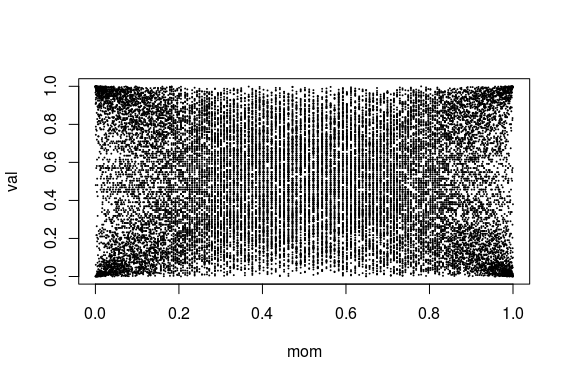
\includegraphics[scale=1]{obs}
\caption{Pseudo-Observations of the returns plotted against each other}
\end{figure}
\begin{figure}
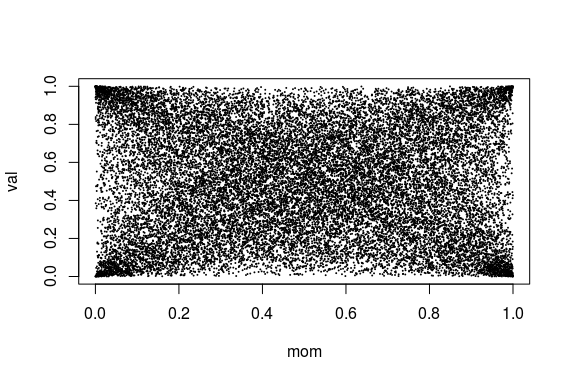
\includegraphics[scale=1]{res}
\caption{Pseudo-Observations of the residuals plotted against each other}
\end{figure}
\begin{figure}
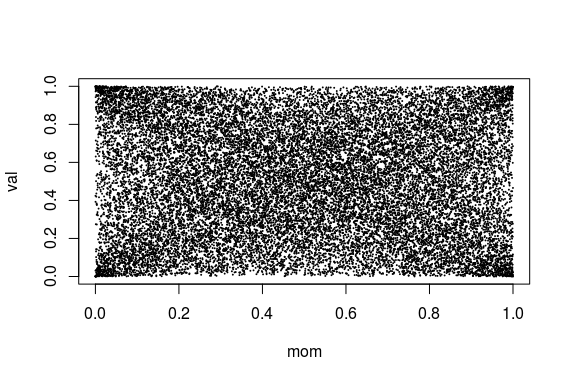
\includegraphics[scale=1]{stres}
\caption{Pseudo-Observations of the standardized residuals plotted against each other}
\end{figure}
% latex table generated in R 3.2.5 by xtable 1.8-2 package
% Sat May  7 14:09:15 2016
\begin{table}[ht]
\centering
\caption{Correlation of standardized residuals}
\begin{tabular}{rrr}
  \hline
 & mom & val \\ 
  \hline
mom & 1.00 & -0.03 \\ 
  val & -0.03 & 1.00 \\ 
   \hline
\end{tabular}
\end{table}
% latex table generated in R 3.2.5 by xtable 1.8-2 package
% Sat May  7 16:37:46 2016
\begin{table}[ht]
\centering
\caption{T Scores with robust standard errors (momentum)}
\begin{tabular}{rr}
  \hline
 & T Score \\ 
  \hline
mu & 10.41 \\ 
  ar1 & 31.76 \\ 
  ar2 & -61.60 \\ 
  ar3 & -13.31 \\ 
  ar4 & 102.47 \\ 
  ar5 & -1.33 \\ 
  ma1 & -20.87 \\ 
  ma2 & 38.10 \\ 
  ma3 & 29.30 \\ 
  ma4 & -72.64 \\ 
  ma5 & -1.06 \\ 
  omega & -4.08 \\ 
  alpha1 & -10.15 \\ 
  alpha2 & -9.00 \\ 
  alpha3 & 10.26 \\ 
  alpha4 & 11.30 \\ 
  alpha5 & 11.61 \\ 
  beta1 & 30.00 \\ 
  beta2 & 2684035.13 \\ 
  beta3 & 5247674.16 \\ 
  beta4 & 182.88 \\ 
  beta5 & -288567276.16 \\ 
  gamma1 & 4.87 \\ 
  gamma2 & 3.17 \\ 
  gamma3 & 11.93 \\ 
  gamma4 & -4.69 \\ 
  gamma5 & -3.39 \\ 
  skew & 109.34 \\ 
  shape & 19.51 \\ 
   \hline
\end{tabular}
\end{table}
% latex table generated in R 3.2.5 by xtable 1.8-2 package
% Sat May  7 16:40:19 2016
\begin{table}[ht]
\centering
\caption{T Scores with robust standard errors (value)}
\begin{tabular}{rr}
  \hline
 & T Score \\ 
  \hline
mu & 0.61 \\ 
  ar1 & 7.41 \\ 
  ar2 & -3.99 \\ 
  ar3 & 8.50 \\ 
  ar4 & 0.11 \\ 
  ar5 & -0.31 \\ 
  ma1 & -3.78 \\ 
  ma2 & 2.35 \\ 
  ma3 & -1.82 \\ 
  ma4 & -0.14 \\ 
  ma5 & 0.37 \\ 
  omega & -6.55 \\ 
  alpha1 & 0.14 \\ 
  alpha2 & 0.44 \\ 
  alpha3 & -0.73 \\ 
  alpha4 & -0.09 \\ 
  alpha5 & -0.15 \\ 
  beta1 & 5705.46 \\ 
  beta2 & 3540.51 \\ 
  beta3 & 4454.70 \\ 
  beta4 & -19455.86 \\ 
  beta5 & -868607.49 \\ 
  gamma1 & 2554.68 \\ 
  gamma2 & 2.90 \\ 
  gamma3 & -2.81 \\ 
  gamma4 & -2397.56 \\ 
  gamma5 & -0.94 \\ 
  skew & 50.90 \\ 
  shape & 11.73 \\ 
   \hline
\end{tabular}
\end{table}
\begin{figure}
\includegraphics[scale=1]{qqplotmom}
\caption{Q-Q Plot of Standardized Residuals (Momentum)}
\end{figure}
\begin{figure}
\includegraphics[scale=1]{qqplotval}
\caption{Q-Q Plot of Standardized Residuals (Value)}
\end{figure}
\end{document}